\chapter{Computed Tomography (CT)}

Computed Tomography (CT) is a medical imaging modality that became
clinically available in the early 1970s and was the first to be made
possible by computers. CT can provide isotropic\footnote{Isotropic
  spatial resolution is a characteristic of images where the
  resolution is equal in all directions. In the case of 3D images,
  this means that a voxel (a 3D pixel) is a perfect cube, with equal
  dimensions on all sides.: along the X-axis (left-right), the Y-axis
  (up-down), and the Z-axis (front-back). } 3D images (volumes),
including axial\footnote{An axial view divides the body horizontally
  into a top (superior) and bottom (inferior) section.},
coronal\footnote{A coronal view divides the body vertically into a
  front (anterior) and back (posterior) section.}, and
sagittal\footnote{A sagittal view divides the body vertically into a
  right and left section.} views. The images are obtained by X-ray
transmission, moving an X-ray tube (the gantry) and detector arrays
around the patient(see Figure~\ref{fig:views_in_CT}).

\begin{figure}
  \centering
  \begin{tabular}{cc}
    \href{https://www.ahajournals.org/doi/10.1161/01.cir.0000048965.56529.c2}{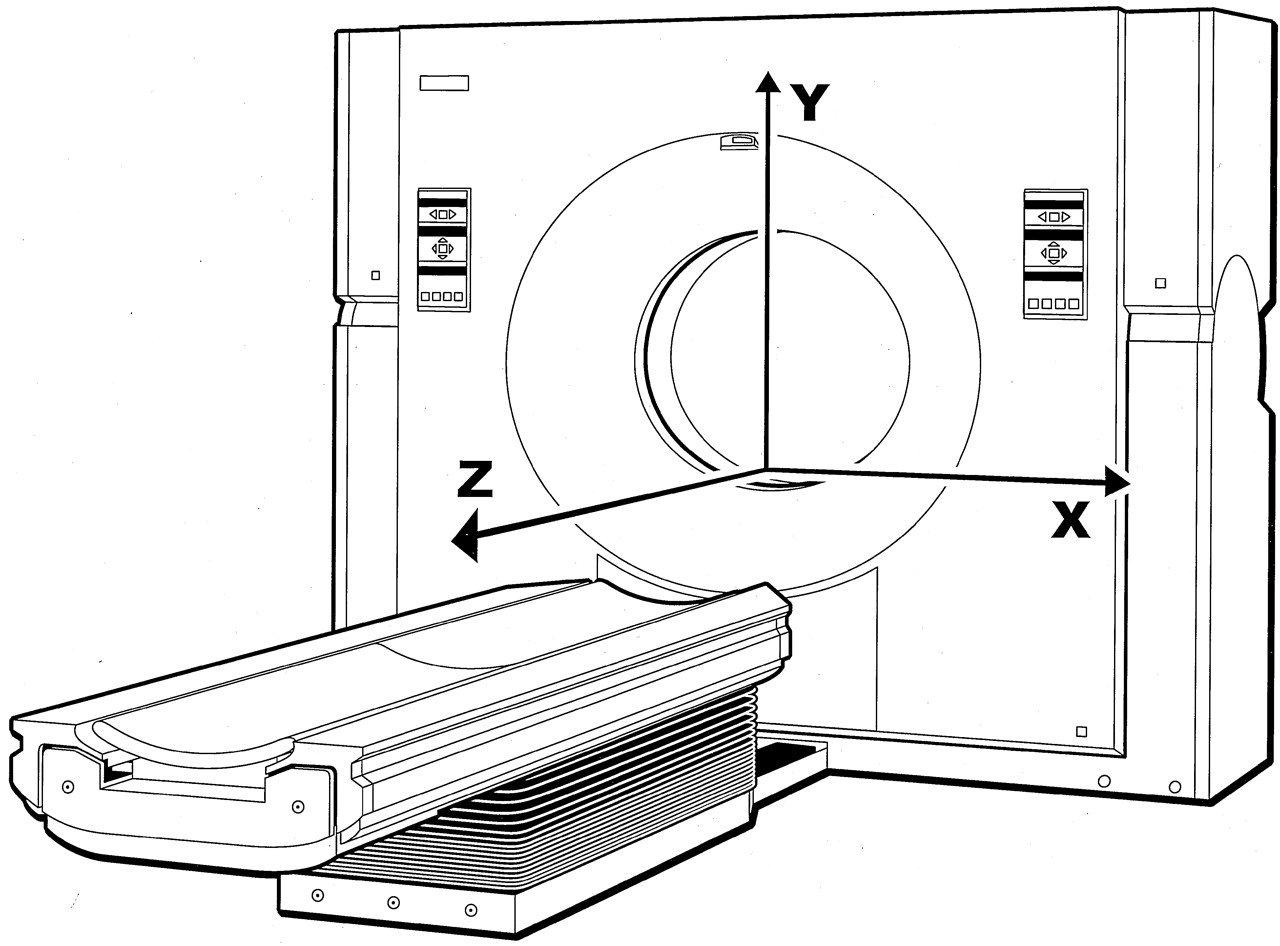
\includegraphics{CT_axis__www.ahajournals.orgdoi10.116101.cir.0000048965.56529.c2~.jpeg}} & 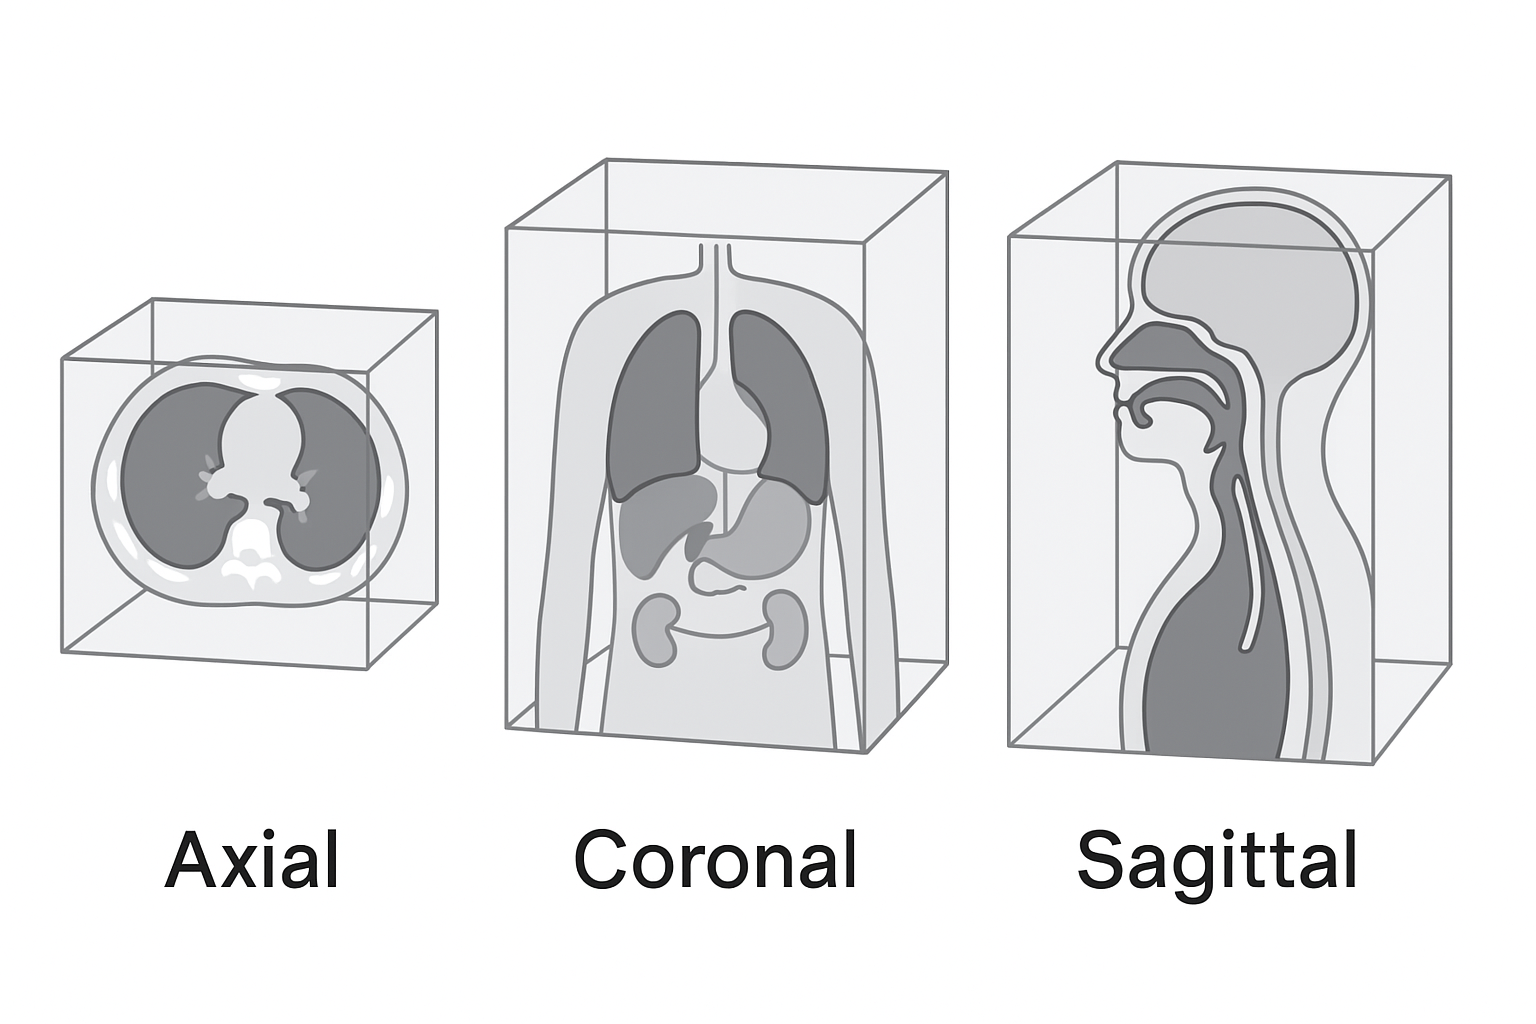
\includegraphics{axial_coronal_sagittal}
  \end{tabular}
  \caption{Reference axis used in CT and type of views generated.\label{fig:views_in_CT}}
\end{figure}

\section{Acquisition}

\begin{figure}
  \centering
  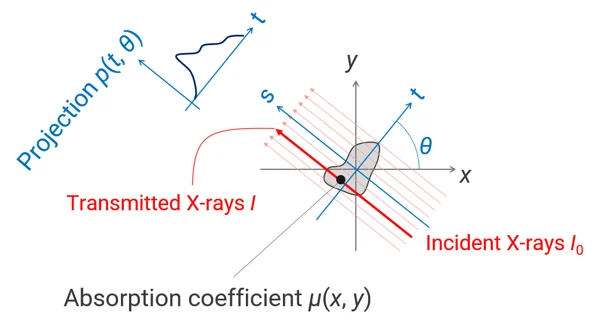
\includegraphics{projection}
  \caption{A projection example \cite{takase2025CT}. $\theta$ is the
    angle used for taking the projection and $t$ the location in
    the detector.\label{fig:projection}}
\end{figure}

The 2D data collected from each angle is called a \emph{projection}
(see Figure~\ref{fig:projection}), consisting of multiple individual
attenuation measurements. The acquisition process can be classified as
(see Figure~\ref{fig:CT_geometries}):

\begin{figure}
  \centering
  \includegraphics{geometries}
  \caption{Geometries used in CT \cite{takase2025CT}.\label{fig:CT_geometries}}
\end{figure}

\begin{enumerate}
\item \textbf{Parallel-beam acquisition}: The X-rays are parallel
  (usually using a collimator) and the detector is organized as a 1D
  array.

\item \textbf{Fan-beam acquisition}: The X-rays form a fan with the vertice in the emitter
  in a line (using a collimator) and the detector is organized as a 1D
  array.

\item \textbf{Cone-beam acquisition}: The X-rays form a cone with the
  vertice in the emitter, and the detector is a 2D array.
  
\end{enumerate}

\begin{figure}
  \centering
  \begin{table}{cc}
    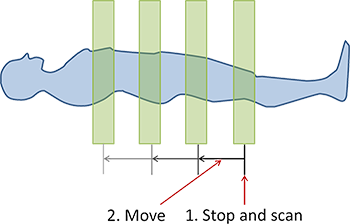
\includegraphics{axial_scanning} & 
\includegraphics{helical_scanning}
  \end{table}
  \caption{Types of scanning used in CT \cite{abdulla2025acquiring1}.\label{fig:scannings}}
\end{figure}

Depending on how the scanning is performed, we can distinguish between
(see Figure~\ref{fig:scannings}):

\begin{enumerate}
\item \textbf{Axial (sequential) scanning}:
  The gantry completes a 360-degree rotation to acquire projection
  data while the patient table is stationary. 

\item \textbf{Helical (spiral) scanning}: The patient table moves
  at a constant speed while the gantry rotates, causing the X-rays
  source to form a helix around the patient.
\end{enumerate}

\section{Image reconstruction}
The CT scaner generates a collection (usually thousands) of
projections that need to be processed to obtain the 3D
reconstruction. In parallel- and fan-beam scaners, the projections are
(1D) lines and the set of all projections for the same Z-plane form a
2D image called \emph{sinogram}
\cite{wikipedia2025radom_transform}\footnote{The Radon transform
  describes how CT projections are mathematically related to the
  scanned object; back-projection is the reconstruction method that
  (with filtering) approximates the inverse Radon transform to recover
  the object from its projections.}. In cone-beam scaners, the
sinogram is a 3D cube.

To generate the 3D reconstruction, the following tasks are usually done:

\begin{enumerate}
\item \textbf{Calibration}: A phantom patient (that we know exactly
  its morphology) is used to test if the reconstructions have some
  problem, such as for example, the detector sensitivity (affects to
  the contrast), ``dead-pixels'' in the detector (that should be
  interpolated), etc. This task should be performed periodically.
\item \textbf{Denoising}: The sinograms used to be quite
  smooth. Therefore, some technique for removing noise can be
  useful. This task is performed in every scan.
\item \textbf{Logarithmic transformation}: The X-rays are
  exponentially attenuated when they travel across the tissues. This
  step converts the rest of task in a linear operation.
\item \textbf{Filtered BackProjection (FBP)}: A 3D reconstruction
  matrix accumulates in each voxel the constribution of each
  projection, that previously has been filtered using a high-pass
  filter to sharpen the textures of the reconstruction. Such filtering
  is usually performed in the Fourier domain, where the convolution is
  a linear-time operation.\footnote{The FFT (Fast Fourier Transform,
    both forward and inverse) is $\mathcal{O}(n\log_2(n))$ and the
    multiplication is $\mathcal{O}(n)$, where $n$ is the number of
    elements to convolve. Convolution in the signal domain is
    $\mathcal{O}(n^2)$. Therefore, for large enough $n$, convolution
    in the Fourier domain is faster.}
  
    ◦ Simple Backprojection: The simplest method of reconstruction, backprojection, involves "smearing" the measured projection values back into the image matrix
. However, this leads to a characteristic 1/r blurring artifact in the reconstructed image
.
    ◦ Filtered Backprojection (FBP): To correct for the blurring caused by simple backprojection, mathematical filters (known as reconstruction kernels) are applied to the projection data before backprojection
. These filters, such as the "ramp" filter or "roll-off" filters (e.g., Shepp-Logan, Hamming, Cosine, or vendor-specific names like "soft tissue" or "bone" filters), are designed to enhance spatial frequencies and manage image noise. Fourier transforms are often used to perform these filtering operations more quickly
.
    ◦ Iterative Reconstruction: Increasingly common in modern CT, iterative reconstruction algorithms are numerically intensive and involve a series of computational steps
. These algorithms start with an initial guess of the image, calculate forward projections, compare them to the actual measured projection data to generate an "error matrix," and then use this error to update the image in successive iterations until an accurate depiction of the scanned object is achieved. Iterative methods can model various physical parameters that FBP cannot, leading to images with higher signal-to-noise ratio (SNR) at the same dose, or comparable SNR at lower doses
.
4. Image Display and Analysis
    ◦ Hounsfield Units (HU): The quantitative gray scale values in CT images are known as Hounsfield units (HUs), named after Sir Godfrey Hounsfield, a key innovator in early CT technology
. HUs are derived from the linear attenuation coefficient of a tissue relative to water, with water defined as 0 HU and air as -1000 HU. Different tissues and materials have characteristic HU ranges, allowing for quantitative assessment of anatomical structures
.
    ◦ Voxel and Pixel: The 3D cross-section of tissue corresponding to a CT image is referred to as a volume element (voxel), while each picture element in the 2D reconstructed image is called a pixel
.
5. Advanced Applications
    ◦ CT Angiography (CTA): This involves contrast-enhanced CT scans where images are processed to highlight vascular anatomy, providing less invasive diagnostic procedures than traditional angiography
.
    ◦ CT Perfusion: Used to evaluate blood flow and vascular function within organs (e.g., the brain during stroke evaluation), involving repeated real-time imaging of an organ after contrast administration
.
    ◦ Dual Energy CT: This technique acquires X-ray data at two different energy levels (kV) to differentiate materials based on their elemental composition, allowing for improved tissue characterisation
.

quantum noise



The output of this
process is a \emph{sinogram}, a 3D array of data in which one
dimension represents the angle of the corresponding sinogram-slice,
and the other two dimensions


CT volumes are produced by passing
X-rays through the body at a large number of angles. The numerous
slices collected in this manner (forming a sinogram) which is
transformed into a tomographic\footnote{The term tomography refers to a
  picture (graph) of a slice (tomo).} image (a volume) of the
patient \cite{bushberg2011essential}.

The advantage of CT over radiography is its ability to display
three-dimensional (3D) slices of the anatomy of interest, eliminating
the superposition of anatomical structures and thereby presenting an
unobstructed view of detailed anatomy to the physician
\cite{bushberg2011essential}.

While CT is usually used for anatomic imaging, the use of
iodinated contrast injected intravenously allows the functional
assessment of various organs as well \cite{bushberg2011essential}.

To transform a sinogram into a tomogram there is basically two mathematical tools:
\begin{enumerate}
\item Radon transform (also called the \emph{filtered back-projection
    method}) \cite{wikipedia2025radom_transform}.
\item Iterative reconstruction.
\section{Image quality}

Emphasis on iterative reconstruction for improved SNR and dose
reduction compared to filtered backprojection. Dual energy CT and its
reconstruction approaches, including logarithmic weighted
subtraction. CT Perfusion generating pseudocolored parametric maps
(blood volume, perfusion) from time-series images using mathematical
models. Tube current modulation for dose optimisation and homogeneous
noise distribution

In X-ray and gamma-ray imaging, SNR is improved by collecting more
photons (quanta), increasing acquisition time, or source intensity
\cite{bushberg2011essential}.


Iterative reconstruction in CT and SPECT can significantly reduce
image noise at lower doses \cite{bushberg2011essential}.

Radon transform


\section{Resources}

\bibliography{tomography}
